\documentclass{ximera}

\title{Insight}

\begin{document}
\begin{abstract}
The insight portion of the self-evaluation test for the University of
Leuven's Masters of Artificial Intelligence program.
\end{abstract}
\maketitle


% Question 35
\begin{question}
A clique is  a fully connected subset of nodes in a graph. 
A maximal clique is a clique which is not a subset of a larger clique.
Consider now the graph below, where the $X_i$ are the nodes.  What are the maximal cliques? 
\begin{image}
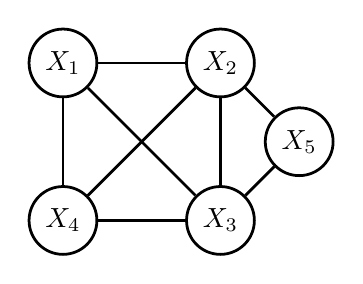
\begin{tikzpicture}[line width=1.5pt,circle, draw,thick,minimum size=6mm,line width=1pt,>=stealth]
%\node[font=\Large] at (1.2,2.8) {Undirected Graph};
\node[circle, draw,thick,minimum size=6mm,line width=1pt,>=stealth] (x1) at (0,2) {$X_1$};
\node[circle, draw,thick,minimum size=6mm,line width=1pt,>=stealth] (x2) at (2,2) {$X_2$};
\node[circle, draw,thick,minimum size=6mm,line width=1pt,>=stealth] (x3) at (2,0) {$X_3$};
\node[circle, draw,thick,minimum size=6mm,line width=1pt,>=stealth] (x4) at (0,0) {$X_4$};
\node[circle, draw,thick,minimum size=6mm,line width=1pt,>=stealth] (x5) at (3,1) {$X_5$};
\draw(x1) -- (x2);\draw(x1) -- (x3); \draw(x1) -- (x4);
\draw(x2) -- (x3); \draw(x2) -- (x4);
\draw(x3) -- (x4); \draw(x2)--(x5);\draw(x3)--(x5);
\end{tikzpicture}
\end{image}

\begin{solution}%% Make multiple choice
\begin{multiple-choice}
\choice{$\{X_1,X_2,X_4\}$}
\choice[correct]{$\{X_2,X_3,X_5\}$}
\choice[correct]{$\{X_1,X_2,X_3,X_4\}$}
\end{multiple-choice}
\end{solution}
\end{question}

% Question 36
\begin{question}
Consider the following definitions.  
A vertical bar separates alternatives. For instance, $gray  \mid grey$ defines the set \{$gray$, $grey$\}.
Parentheses are used to define the scope and precedence of the operators (among other uses). For example, $gray \mid grey$ and $gr(a\mid e)y$ are equivalent patterns which both describe the set 
 \{$gray$, $grey$\}.
The quantifier $^*$ denotes that the previous element may be repeated zero or more times. 
 For example, $ab^*c$ includes $ac$, $abc$, $abbc$, $abbbc$, and so on.

Which of the following elements are included in the set $d (a \mid bc)^*t  $ ?
Does the set  include $dat$, $daaaaat$, $dbcabct$ ?  

\begin{solution}
\begin{multiple-choice}
\choice[correct]{$dat$}
\choice[correct]{$daaaaat$}
\choice[correct]{$dbcabct$}
\end{multiple-choice}
\end{solution}
 
All three strings match the given expression:
\begin{align*}
&d \, \underline{a} \, t\\
&d \, \underline{a} \, \underline{a} \, \underline{a} \, \underline{a} \, \underline{a} \, t\\
&d \, \underline{bc} \, \underline{a} \, \underline{bc} \, t
\end{align*}
\end{question}

% Second part of question 36
\begin{question}
How would you define the set of all binary representations of natural numbers (i.e., 0, 1, 10, 11, ... ) using the definitions given in previous question?

\begin{solution}%% Make multiple choice
The answer is \answer{$0 | (1(0|1)*)$}.
\end{solution}
\end{question}

\end{document}
